\section{結果}
項目ごとに,CUDに配慮した工夫が取り入れられていた資料の割合を図\ref{fig:result}に示す.

配色に関する項目について,
強調目的の色でCUDに配慮されていた資料は90%であり,先行研究に比べて10ポイント増加している.
色の組み合わせでは,全ての資料がCUDに配慮した配色となっていた.

色以外の工夫に関する項目について,
適切なフォントでは,全ての資料がCUDに配慮したフォントとなっていた.
また,ハッチングでCUDに配慮されていた資料は90%であった.
一方,新たに評価項目として加えた装飾でCUDに配慮されていた資料は70%であった.

\begin{figure}[h]
\begin{center}
 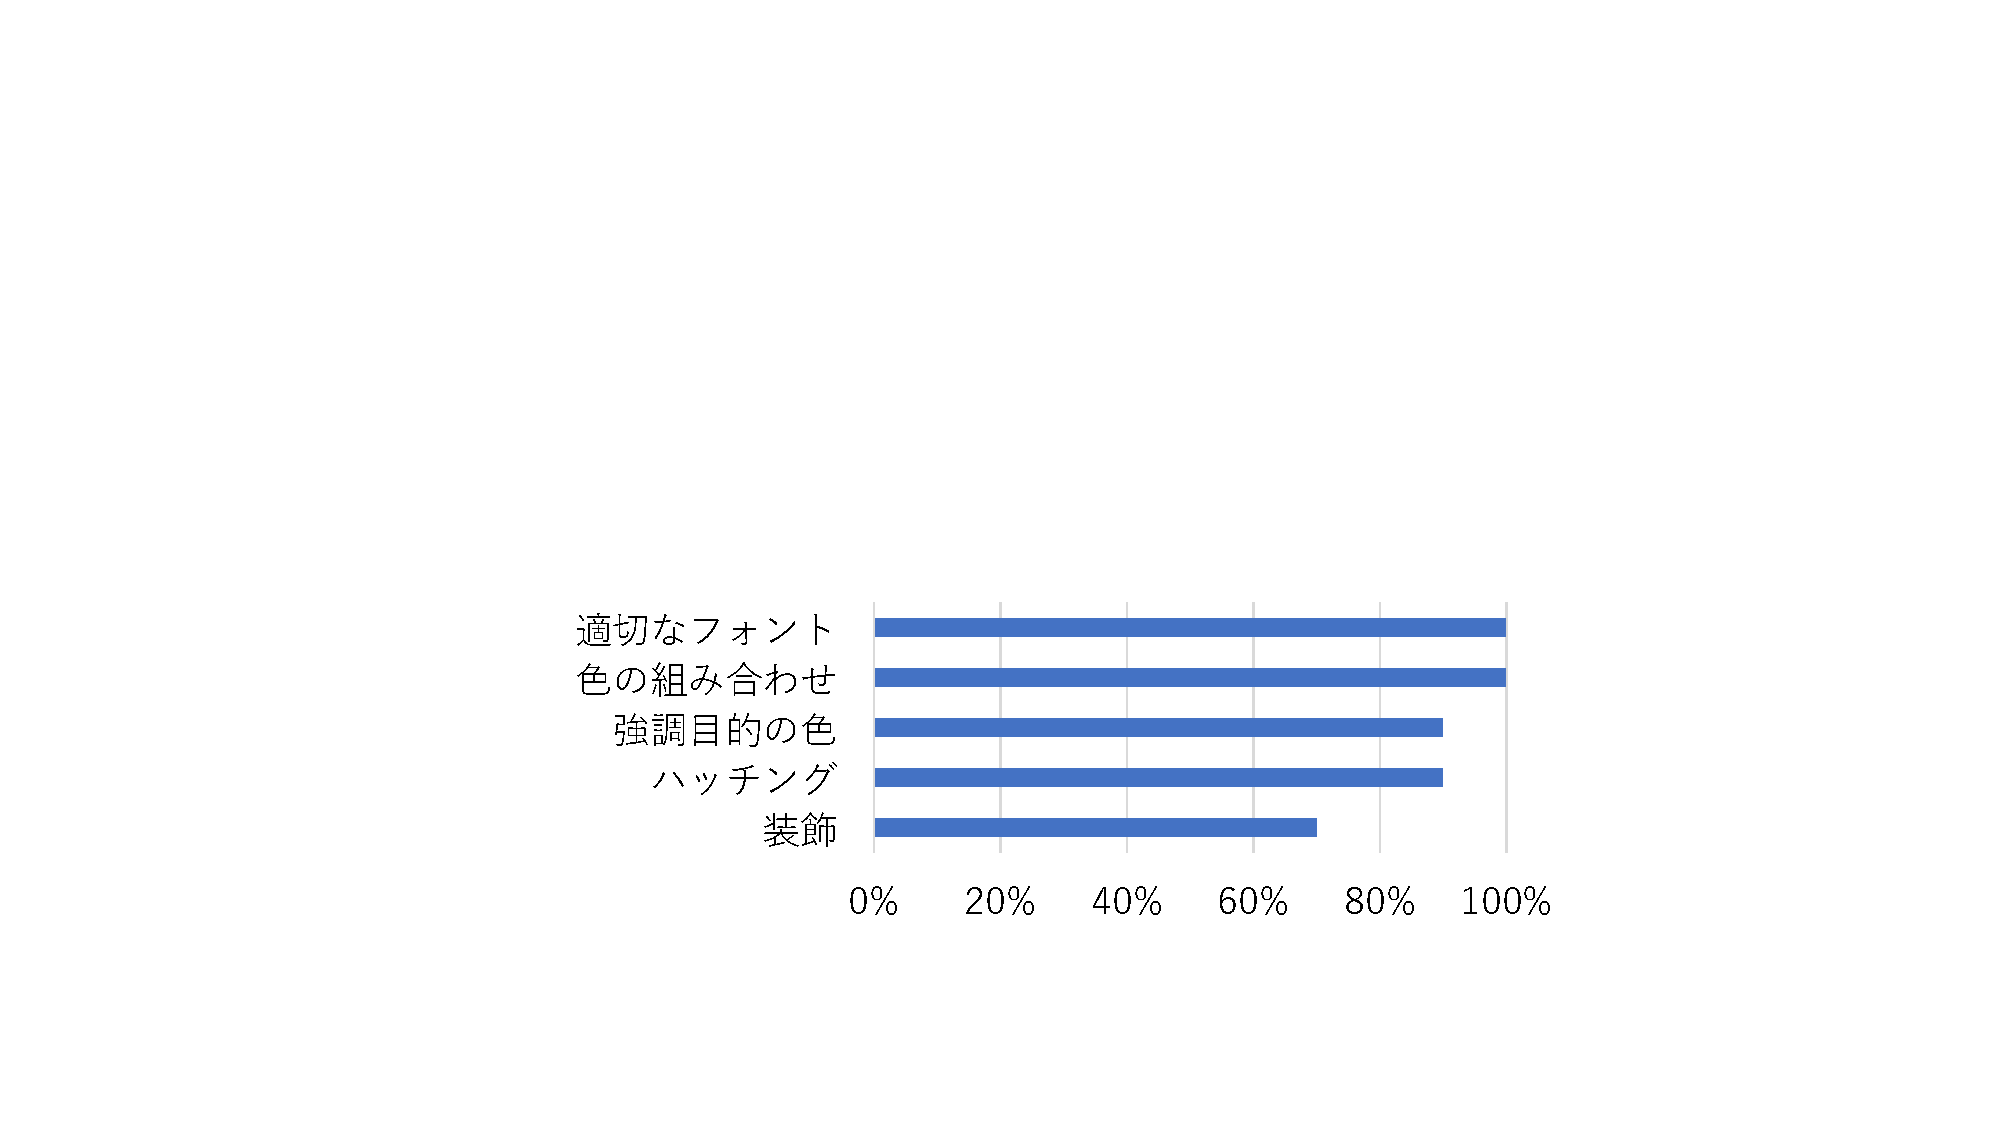
\includegraphics[clip,width=110mm,height=38mm]{images/result.pdf}
\end{center}
 \caption{CUD評価結果}
 \label{fig:result}
\end{figure}
